\section{Markov/Undirected Graphical Models}

\begin{frame}{Gibbs Distribution}
\begin{definition}[Factor, Clique Potential]
    Let $\mathcal{S} \subseteq \mathcal{X} = (X_1,\ldots,X_n)$ be a set of random variables with label spaces $L_{X_1},\ldots,L_{X_n}$.
    We define a factor (also called clique potential) $\phi$ to be a function from $\prod_{X \in \mathcal{S}} L_{X}$ to $\R$.
    A factor is nonnegative if all its entries are nonnegative.
    The set of variables $\mathcal{S}$ is called the scope of the factor and is denoted by $\Scope[\phi]$.
\end{definition}
\begin{itemize}
    \pause \item A factor will denote the compatibility between variables in its scope. High values correspond to likely combinations of values.
\end{itemize}
\pause
\begin{definition}[Gibbs Distribution]
   Let a set of factors $\Phi = \{\phi_1,\ldots,\phi_m\}$ be given with $\Scope[\phi_1] \cup \ldots \cup \Scope[\phi_m] = \{X_1,\ldots,X_n\}$.
   We define the probability distribution and partition function as
   \begin{align}
    \Pb_{\Phi}[X_1,\ldots, X_n] & = \frac{1}{Z} \prod_{i=1}^k \phi_i\left(X_{\Scope[\phi_i]}\right),
&
    Z & = \sum_{X_1,\ldots,X_n} \prod_{i=1}^k \phi_i\left(X_{\Scope[\phi_i]}\right)\,.
   \end{align}
%   where the partition function is defined as
%   \begin{equation}
 %  \end{equation}
\end{definition}
\begin{itemize}
    \pause \item The overall probability distribution is proportional to the product of all factors.
    \pause \item The partition function ensures that the distribution is normalized.
\end{itemize}
\end{frame}

\begin{frame}{Markov/Undirected Graphical Models}
\begin{definition}[Markov Network]
    A Gibbs distribution $\Pb_{\Phi}$ factorizes over an undirected graph (referred to as Markov Network) if for each factor $\phi_i$ the scope $\Scope[\phi_i]$ is a clique in the graph.
\end{definition}
\begin{minipage}{0.6\textwidth}
\begin{itemize}
    \pause \item Can we go from Markov network structure to determine the scopes of the potentials? 
    \begin{itemize}\pause \item No, consider $\{\textcolor{blue}{\phi_1},\textcolor{green}{\phi_2},\textcolor{orange}{\phi_3}\}$ with $\Scope[\textcolor{blue}{\phi_1}] = \{X_1,X_2\}$, $\Scope[\textcolor{green}{\phi_2}] = \{X_2,X_3\}$, $\Scope[\textcolor{orange}{\phi_3}] = \{X_1,X_3\}$ and $\Phi' = \{\textcolor{red}{\phi'}\}$ with $\Scope[\textcolor{red}{\phi'}] = \{X_1,X_2,X_3\}$.
    \end{itemize}
\end{itemize}
\vspace{0.2cm}
\end{minipage}
\begin{minipage}{0.36\textwidth}
\begin{tikzpicture}[scale=0.7]
\begin{scope}[shift={(3.5,0)}]
    \only<8->{
        \draw[fill=red!80,nearly transparent, rounded corners] (-1.5,0.5) -- (-1.5,-0.5) -- (-0.5,-1.65)  -- (0.5,-1.65)  -- (1.5,-0.5) -- (1.5,0.5) -- cycle;
\node[rand_var] (X1) at (-1,0) {$X_1$};
\node[rand_var] (X2) at (0,-1.15) {$X_2$};
\node[rand_var] (X3) at (1,0) {$X_3$};
\draw[thick] (X1) -- (X2);
\draw[thick] (X1) -- (X3);
\draw[thick] (X2) -- (X3);
    }
\end{scope}
%
    \only<4,7->{\draw[fill=blue!80, nearly transparent, rounded corners] (-1.5,0.5) -- (-1.5,-0.5) -- (-0.5,-1.65)  -- (0.5,-1.65)  -- (0.5,-0.65) -- (-0.5,0.5) -- cycle;}
    \only<5,7->{\draw[fill=green!80,nearly transparent, rounded corners] (-0.5,-0.65) -- (-0.5,-1.65)  -- (0.5,-1.65)  -- (1.5,-0.5) -- (1.5,0.5) -- (0.5,0.5) -- cycle;}
    \only<6,7->{\draw[fill=orange!80,nearly transparent, rounded corners] (-1.5,0.5) -- (-1.5,-0.5) -- (1.5,-0.5) -- (1.5,0.5) -- cycle;}
\node[rand_var] (X1) at (-1,0) {$X_1$};
\node[rand_var] (X2) at (0,-1.15) {$X_2$};
\node[rand_var] (X3) at (1,0) {$X_3$};
\draw[thick] (X1) -- (X2);
\draw[thick] (X1) -- (X3);
\draw[thick] (X2) -- (X3);
\end{tikzpicture}
\end{minipage}

\pause \pause \pause \pause \pause \pause
\begin{definition}[Pairwise Markov Network]
A pairwise Markov network is a Markov network where $\abs{\Scope[\phi]} = 2$ for all factors $\phi$.
\end{definition}
\end{frame}

\begin{frame}{Pairwise Markov Network Examples}
    A pairwise Markov network can be written as product of unary and pairwise factors
\begin{equation}
    \Pb[X_1,\ldots,X_n] = \underbrace{\prod_{i=1}^n \phi_i(X_i)}_{\text{unary factors}} \underbrace{\prod_{ij \in E} \phi_{ij}(X_i,X_j)}_{\text{pairwise factors}}
\end{equation}
\pause

\begin{example}[Pairwise Markov Networks in Computer Vision]
\begin{center}
    \begin{figure}
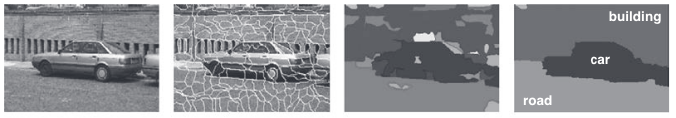
\includegraphics[width=0.9\textwidth]{img/Markov-network-computer-vision.png}
    \caption{Markov Random Fields for Computer Vision: Pairwise connections between adjacent superpixels for compatibility of segmentation labels.}
    \end{figure}
\end{center}
\begin{itemize}
    \item Nodes $\leftrightarrow$ (super-)pixels.
\item Unary factors: compatibility between pixel and class assignment.
\item Pairwise factors: compatibility between neighboring pixels (are they similar $\Rightarrow$ prefer same class assignment of both).
\end{itemize}
\end{example}
\end{frame}


\begin{frame}{Independencies, Soundness, Factorization $\Rightarrow$ I-Map}
\begin{definition}[Separation]
    A set of nodes $Z$ separates $X$ and $Y$ in a Markov network $H = (\mathcal{X},E)$ if there is no path between nodes in $X$ and $Y$ that does not intersect with $Z$.
    We define the global independencies of $H$ as 
    \begin{equation}
        \mathcal{I}(H) = \{(X \indep Y | Z) \mid Z \text{ separates } X \text{ and } Y\}\,.
    \end{equation}
\end{definition}
\pause
\begin{theorem}[Soundness of Separation]
    Let $\Pb$ be a Gibbs distribution that factorizes over $H = (\mathcal{X},E)$, then $H$ is an I-map for $\Pb$.
\end{theorem}
\pause
\begin{proof}
Let $X$, $Y$ and $Z$ be three disjoint subsets such that $Z$ separates $X$ and $Y$.
Assume $X \cup Y \cup Z = \mathcal{X}$.
\pause
As $Z$ separates $X$ and $Y$ there are no direct edges between $X$ and $Y$.
\pause
Hence any clique in $H$ is contained in either $X \cup Z$ or in $Y \cup Z$.
\pause
Let $\mathcal{I}_X$ be the indexes of cliques contained in $X \cup Z$ and $\mathcal{I}_Y$ those in $Y \cup Z$.
\pause
Then 
\begin{equation}
    \Pb[X_1,\ldots,X_n] =
     \frac{1}{Z} \prod_{i \in \mathcal{I}_X} \phi_i\left(X_{\Scope[\phi_i]}\right) \prod_{i \in \mathcal{I}_Y} \phi_i\left(X_{\Scope[\phi_i]}\right) 
     \pause 
     = \frac{f(X,Z)}{\sum_{X} f(X,Z)} \frac{g(Y,Z)}{\sum_{Y} g(Y,Z)}
\end{equation}
\pause
Independence follows from the factorization as a common cause Bayesian network.
\pause
Now consider the case that $U = \mathcal{X} \setminus (X \cup Y \cup Z) \neq \emptyset$.
\pause 
Partition $U$ into $U_1$ and $U_2$ such that $Z$ separates $X \cup U_1$ and $Y \cup U_2$.
\pause 
As above, $X,U_1 \indep Y, U_2 | Z$. 
\pause 
The decomposition property~\eqref{appendix:conditional-independence-properties} implies $X \indep Y | Z$.
\end{proof}
\end{frame}

\begin{frame}{Hammersley Clifford, I-Map $\Rightarrow$ Factorization}
\begin{theorem}[Hammersley Clifford Theorem]
    Let $\Pb$ be a positive distribution and $H = (\mathcal{X},E)$ be a Markov network. If $H$ is an I-map for $\Pb$, then $\Pb$ is a Gibbs distribution that factorizes over $H$.
\end{theorem}
%\pause
%\begin{proof}
%    Will be given later.
%\end{proof}
\pause
\begin{itemize}
    \item Proof will be given later.
\end{itemize}
\pause
\begin{example}[Hammersley Clifford Positivity Condition Necessary]
Let $X_1,\ldots,X_4$ be random binary variables giving probability $1/8$ to
\begin{equation}
\begin{array}{c}
    (0,0,0,0)\quad(1,0,0,0)\quad(1,1,0,0)\quad(1,1,1,0) \\%\quad
    (0,0,0,1)\quad(0,0,1,1)\quad(0,1,1,1)\quad(1,1,1,1)
\end{array}
\end{equation}
and $0$ to all other configurations.
Let $H$ be the graph $X_1 - X_2 - X_3 - X_4 - X_1$.
Then $\Pb$ satisfies independence properties associated with $H$ but $\Pb$ does not factorize according to $H$.
\end{example}
\begin{proof}
\begin{itemize}
    \pause \item Global independencies hold:
Consider $X_1 \indep X_3 | X_2, X_4$.
\pause
For $X_2 = 1, X_4 = 0$ only $X_1 = 1$ will have probability $>0$, thus $\Pb[X_1 = 1 | X_2=1, X_4=0] = 1$ and $X_1$ is trivially independent of $X_3$ given $X_2,X_4$.
\pause
Similar holds true for all other cases, hence global independencies hold.
\pause
\item $\Pb$ does not factorize:
Assume 
$\Pb = \phi_{12}(X_1,X_2) \phi_{23}(X_2,X_3) \phi_{34}(X_3,X_4) \phi_{14}(X_1,X_4)$, i.e. $\Pb$ factorizes according to $H$.
\pause
Since for any state of $X_1,X_2$ there exists states of $X_3,X_4$ that have positive probability, $\phi_{12} > 0$ must hold.
\pause
Similarly $\phi_{23},\phi_{34},\phi_{14} > 0$, which implies $\Pb > 0$.
\end{itemize}
\end{proof}
\end{frame}

\begin{frame}{Completeness of Separation}
\begin{theorem}[Completeness]
Let $H$ be a Markov network structure.
If $X$ and $Y$ are not separated given $Z$ in $H$, then $X$ and $Y$ are dependent given $Z$ in some distribution $\Pb$ that factorizes over $H$.
\end{theorem}
\pause
\begin{proof}
We construct a suitable distribution $\Pb$.
We assume w.l.o.g.\ that all random variables are binary.
\pause
Since $X$ and $Y$ are not separated, there exists a path $X = U_1 - \dots - U_k = Y$ not blocked by $Z$. Choose a minimal length such path.
\pause 
For any $i$ there exists a clique $C_i$ with $U_i, U_{i+1} \in C_i$.
\pause
Define $\phi_{C_i}(X_{\Scope[\phi_{C_i}]}) = \begin{cases} W, & U_i = U_{i+1} \\ 0,& \text{otherwise} \end{cases}$ with $W \gg 0$.
\pause
Note that $C_i \neq C_{i+1}$, since otherwise the path would not be a shortest one.
\pause
All other cliques are uniformly $1$.
\pause
In this distribution $X$ and $Y$ are dependent and the factorization respects $H$.
\end{proof}
\end{frame}

\begin{frame}{Local Independencies}
    \begin{itemize}
    \item Local independencies analoguous to the Bayesian case.
    \item But they are weaker than the global independencies!
    \end{itemize}
    \pause
\begin{definition}[Pairwise Independence]
    Let $H$ be a Markov network.
    We define the pairwise independencies associated with $H$ to be
    \begin{equation}
    \mathcal{I}_p(H) = \{ X \indep Y | \mathcal{X} \backslash \{X,Y\} : \{X,Y\} \notin E)\,.
    \end{equation}
\end{definition}
    \pause
    \begin{definition}[Markov Blanket Independencies]
        For a graph $H$ we define the Markov blanket $\MB_H(X)$ as the neighbors of $X$.
        We define the local independencies associated with $H$ to be
        \begin{equation}
        \mathcal{I}_l(H) = \{X \indep \mathcal{X} \backslash \{X\} - \MB_H(X) | \MB_H(X)\}\,.
        \end{equation}
    \end{definition}
    \begin{itemize}
    \item Trivially $\mathcal{I}_p(H) \subseteq \mathcal{I}_l(H) \subseteq \mathcal{I}(H)$, hence global implies local which in turn implies pairwise independency
    \item Under positivity assumption all three independency definitions are equivalent.
    \end{itemize}
\end{frame}

\begin{frame}{Equivalence of Dependency Definitions}
\begin{theorem}[Pairwise $\Rightarrow$ Global Independency]
Let $\Pb$ be a positive distribution. 
If $\Pb$ satisfies $\mathcal{I}_p(H)$ then it satisfies $\mathcal{I}(H)$.
\end{theorem}
\pause
\begin{proof}
    We want to prove that $X \indep Y | Z$ whenever $Z$ separates $X$ and $Y$.
    We proceed by reverse induction in the size of $Z$.
    \pause
    For $\abs{X} = n-2$ the global independency reduces to the pairwise one.
    \pause 
    Let now $\abs{Z} = k-1$ and let the theorem hold for any $Z'$ with $\abs{Z'} \geq k$.
    \pause
    \begin{itemize}
    \item Case 1: $\abs{X} \geq 2$ or $\abs{Y} \geq 2$. 
    \pause W.l.o.g. $\abs{X} \geq 2$.Choose some $A \in X$.
    It holds that $X \backslash \{A\} \indep Y | Z \cup \{A\}$ due to monotonicity.
    Also $Y$ and $A$ are separated by $Z$, so we have $A \indep Y | Z \cup \mathcal{X} \backslash \{A\}$ by the induction assumption.
    \pause
    Because $\Pb$ is positive, we can apply the intersection property~\eqref{eq:intersection-property} and conclude that
    $X \indep Y | Z$.
    \pause \item Case 2: $\abs{X} = \abs{Y} = 1$.
    \pause
    If $X \cup Y \cup Z = \mathcal{X}$ we refer to the base case.
    \pause Hence there exists an element $A \in \mathcal{X} \backslash (X \cup Y \cup Z)$. 
    \pause If $A$ is not reachable from $Y$ without going over $Z$, by the induction hypothesis it holds that $X \cup \{A\} \indep Y | Z$. By decomposition~\eqref{eq:decomposition-property} we infer $X \indep Y | Z$.
    \pause Analoguously if $A$ is not reachable from $X$.
    \pause The case that $A$ can be reached from both $X$ and $A$ is not possible, since then $Z$ would not separate them.
    \end{itemize}
\end{proof}
\pause
\begin{corollary}
    If $\Pb$ is positive: 
        $\mathcal{I}_p(H)$ is an I-map for $\Pb$
        $\Leftrightarrow$
        $\mathcal{I}_l(H)$ is an I-map for $\Pb$
        $\Leftrightarrow$
        $\mathcal{I}(H)$ is an I-map for $\Pb$.
\end{corollary}
\end{frame}

%\begin{frame}{Log-Linear Models, Energies?}
%\end{frame}


%\begin{frame}{D-Separation $\Leftrightarrow$ Separation in Upward Closure}
%\begin{proof}
%    Let $X$ and $Y$ be separated by $Z$ in the upward closure $G'$.
%    Let $U_1 \Leftrightarrow \ldots \Leftrightarrow U_k$ be a trail in $G$.
%    The trail corresponds to a path in $G'$ after potential shortcutting when using a moral edge.
%\end{proof}
%\end{frame}

\begin{frame}{Energy, Parametrization}
    \begin{definition}[Energy]
    Given a positive Gibbs distribution $\Pb$ with factors $\phi_1,\ldots,\phi_k$ its energy is defined as 
    \begin{equation}
        E(X_1,\ldots,X_n) = \log(\Pb[X_1,\ldots,X_n]) = \sum_{i=1}^k \log(\phi_i(X_{\Scope[\phi_i]}))
    \end{equation}
    We denote energy terms by $\epsilon_i := \log(\phi_i)$.
    \end{definition}
    \pause
\begin{example}[Non-Uniqueness of Parametrizations of Gibbs Distributions]
    \begin{minipage}{0.4\textwidth}
    \begin{center}
    \begin{tikzpicture}
    \node[rand_var] (X1) at (0,3) {$X_1$};
    \node (x11) at (0,0) {$\bullet$};
    \only<5->{\node at (-0.4,0) {\scriptsize$+\delta$};}
    \node (x12) at (0,1) {$\bullet$};
    \node (x13) at (0,2) {$\bullet$};
    \draw (-0.2,-0.2) -- (-0.2,2.2) -- (0.2,2.2) -- (0.2,-0.2) -- cycle;
    \node[rand_var] (X2) at (3,3) {$X_2$};
    \node (x21) at (3,0) {$\bullet$};
    \node (x22) at (3,1) {$\bullet$};
    \node (x23) at (3,2) {$\bullet$};
    \draw (2.8,-0.2) -- (2.8,2.2) -- (3.2,2.2) -- (3.2,-0.2) -- cycle;
    \draw[-] (x11) -- (x21)node[near start, below] {\scriptsize$-\delta$};
    \only<5->{\draw[-] (x11) -- (x21) node[near start, below] {\scriptsize$-\delta$}};
    \draw[-] (x11) -- (x22) node[near start, below] {\scriptsize$-\delta$};
    \only<5->{\draw[-] (x11) -- (x22) node[near start, below] {\scriptsize$-\delta$};}
    \draw[-] (x11) -- (x23) node[near start, below] {\scriptsize$-\delta$};
    \only<5->{\draw[-] (x11) -- (x23) node[near start, below] {\scriptsize$-\delta$};}
    \draw[-] (x12) -- (x21);
    \draw[-] (x12) -- (x22);
    \draw[-] (x12) -- (x23);
    \draw[-] (x13) -- (x21);
    \draw[-] (x13) -- (x22);
    \draw[-] (x13) -- (x23);
    \pause
    \draw[fill=blue!80,nearly transparent, rounded corners]
    (-0.3,-0.3) -- (-0.3,2.3) -- (0.3,2.3) -- (0.3,-0.3) -- cycle;
    \pause
    \draw[fill=green!80,nearly transparent, rounded corners]
    (2.7,-0.3) -- (2.7,2.3) -- (3.3,2.3) -- (3.3,-0.3) -- cycle;
    \pause
    \draw[fill=red!80,nearly transparent, rounded corners]
    (-0.5,-0.5) -- (3.5,-0.5) -- (3.5,2.5) -- (-0.5,2.5) -- cycle;
    \end{tikzpicture}
\end{center}
\end{minipage}
\begin{minipage}{0.59\textwidth}
    Let a Gibbs distribution with $\mathcal{X} = \{X_1,X_2\}$ and factors 
    \begin{itemize}
    \item unary: $\Scope[\textcolor{blue}{\phi_1}] = \{X_1\}$, $\Scope[\textcolor{green}{\phi_2}] = \{X_2\}$,
    \item pairwise: $\Scope[\textcolor{red}{\phi_{12}}] = \{X_1, X_2\}$ 
    \end{itemize}
    be given.
    Let the label space be $L_{X_i} = \{0,1,2\}$.
    Then 
    \begin{itemize}
    \item $\phi_1(x_1) \leftarrow \begin{cases} \phi_1(x_1) + \delta, & x_1 = 0, \\ \phi_{1}(x_1), & \text{otherwise}\end{cases}$
    \item $\phi'_{12}(x_1,x_2) \leftarrow \begin{cases} \phi_{12}(x_1,x_2) - \delta, & x_1 = 0, \\ \phi_{12}(x_1,x_2), & \text{otherwise}\end{cases}$
    \end{itemize}
    produces the same distribution for any $\delta \in \R$.
\end{minipage}
\end{example}
\end{frame}

\begin{frame}{Canonical Parametrization}
    \begin{itemize}
        \item Is there a way to arrive at a unique representative parametrization?
    \end{itemize}
\begin{definition}[Canonical Parametrization]
    Let a positive Gibbs distribution with factors $\phi_1,\ldots,\phi_k$ be given. 
    Fix an arbitrary assignment $\xi^* = (x_1^*, \ldots, x_n^*)$.
    We will refer to factors by specifying their scopes.
    \pause
    For any factor $\phi_i$ add additional factors for any subset $D \subsetneq \Scope[\phi_i]$.
\pause
    The canonical energy function for a clique $D$ is
    \begin{equation}
        \label{eq:canonical-energy-function}
        \epsilon_D(X_D) = \sum_{Z \subseteq D} (-1)^{\abs{D \backslash Z}} \log(\Pb(X_Z, \xi^*_{\mathcal{X} \backslash Z}))\,
    \end{equation}
    where the empty clique $\varnothing$ is also included.
\end{definition}
\begin{itemize}
\pause \item The canonical energy function~\eqref{eq:canonical-energy-function} performs an inclusion/exclusion summation.
\pause \item It is not useful for actual computations, but will help us in the proof of Hammersley Clifford.
\end{itemize}
\pause
\begin{theorem}[Soundness of Canonical Parametrization]
    Let $\Pb$ be a positive Gibbs distribution. The canonical parametrization gives the same probability distribution, i.e.\ 
    \begin{equation}
        \label{eq:canonical-parametrization}
        \Pb[x] = \exp\left(\sum_{i} \epsilon_{i}(x_{\Scope[\epsilon^*_i]})\right)\,.
    \end{equation}
    In particular, its partition function $Z$ is 1.
\end{theorem}
\end{frame}

\begin{frame}{Soundness of Canonical Parametrization, Proof}
\begin{proof}
    First, let $H=(\mathcal{X},E)$ be the complete graph.
\pause
For $Z = \mathcal{X}$ there is exactly one factor $\epsilon_{\mathcal{X}}$ that by construction has one term $\log(\Pb[X_{\mathcal{X}}])$ in $\epsilon_{\mathcal{X}}$.
\pause
For all other $Z \subsetneq \mathcal{X}$ we need to prove $\log(\Pb[X_Z, \xi^*_{\mathcal{X} \backslash Z}])$ appears equally often with negative and positive signs.

\pause 
The term $\log(\Pb[X_Z,\xi^*_{\mathcal{X} \backslash Z}])$ will appear in $\epsilon_D$
\begin{itemize}
\pause \item once, i.e.\ $= \binom{\abs{\mathcal{X}} - \abs{Z}}{0}$ for any $D$ with $\abs{D} = \abs{Z}$ with sign $+1$ (in $\epsilon_Z$),
\pause \item $\abs{\mathcal{X}} - \abs{Z} = \binom{\abs{\mathcal{X}} - \abs{Z}}{1}$ times for any $D$ with $\abs{D} = \abs{Z}+1$ with sign $-1$,
\pause \item $\binom{\abs{\mathcal{X}} - \abs{Z}}{2}$ times for any $D$ with $\abs{D} = \abs{Z}+2$ with sign $+1$,
\pause \item $\ldots$
\end{itemize}
Hence $\log(\Pb[X_Z, \xi^*_{\mathcal{X} \backslash{Z}}])$ appears in sum with coefficient
\begin{equation}
    \sum_{k=0}^{\abs{\mathcal{X}} -\abs{Z}} \binom{\abs{\mathcal{X}} - \abs{Z}}{k} (-1)^k
    \pause = (1 - 1)^{\abs{\mathcal{X}} - \abs{Z}}
    \pause = 0\,
\end{equation}
\pause
The proof for $H$ being not the complete graph will be a by-product of the proof of the Hammersley Clifford theorem.
\end{proof}
\end{frame}

\begin{frame}{Proof of Hammersley Clifford}
\begin{theorem}[Hammersley Clifford Theorem]
    $\Pb$ positive, $H$ a Markov network. $\mathcal{I}(H) \subseteq \mathcal{I}(\Pb)$ $\Rightarrow$ $\Pb$ is a Gibbs distribution that factorizes over $H$.
\end{theorem}
\begin{proof}
    We show existence of a Gibbs parametrization for any distribution $\Pb$ that satisfies the Markov assumption of $H$.
    \pause
    For this, we will construct the Gibbs parametrization using the canonical parametrization.
    \pause
    For any subset $D \subseteq \mathcal{X}$ (also $D$ that are not cliques) define $\epsilon_D$ as in~\eqref{eq:canonical-energy-function}.
    \pause 
    As seen above the resulting Gibbs distribution is $\Pb$.
    \pause
    It remains to show that the distribution factorizes over $H$.
    \pause 
    To this end we show that $\epsilon_D$ are identically zero whenever $D$ is not a clique in $H$.
    \pause 
    Assume we have $X, Y \in D$ such that there is no edge between $X$ and $Y$.
    \pause
    Then for any configuration $d$ of the random variables $\mathcal{X}$
    \begin{equation}
        \epsilon_D(d) = \sum_{Z \subseteq D} (-1)^{\abs{D \backslash Z}} \log(\Pb[d_Z, \xi^*_{\mathcal{X} \backslash Z}])\,.
    \end{equation}
    \pause 
    We rearrange the sum into groups of subsets.
    For $W \subseteq D \backslash \{X,Y\}$ the sets $W$, $W\cup \{X\}$, $W \cup \{Y\}$ and $W \cup \{X,Y\}$ are subsets of $D$.
    \pause
    We can rewrite the above summation as
    \begin{multline}
        \epsilon_D(d) =  \sum_{W \subseteq D \backslash \{X,Y\}} (-1)^{\abs{D \backslash \{X,Y\} \backslash W}} 
        \Big(
        \log(\Pb[d_W, \xi^*_{\mathcal{X} \backslash W}]) 
        - \log(\Pb[d_{W \cup \{X\}}, \xi^*_{\mathcal{X} \backslash (W \cup \{X\})}]) \\
        - \log(\Pb[d_{W \cup \{Y\}}, \xi^*_{\mathcal{X} \backslash (W \cup \{Y\})}])
        + \log(\Pb[d_{W \cup \{X,Y\}}, \xi^*_{\mathcal{X} \backslash (W \cup \{X,Y\})}])
        \Big)
    \end{multline}
\end{proof}
\end{frame}

\begin{frame}{Proof of Hammersley Clifford II}
    \begin{proof}
    Consider a specific $W$ in the above sum. 
    \begin{equation}
    \begin{aligned}
        & \log(\Pb[d_{W \cup \{X,Y\}}, \xi^*_{\mathcal{X} \backslash (W \cup \{X,Y\})}])
        - \log(\Pb[d_{W \cup \{X\}}, \xi^*_{\mathcal{X} \backslash (W \cup \{X\})}])  \\
        \pause = & \log(\frac{\Pb[d_{X}, d_{Y}, d_{W},\xi^*_{\mathcal{X} \backslash D}]}{\Pb[d_{X},\xi^*_{Y},d_{W},\xi^*_{\mathcal{X} \backslash D}]}) \\
        \pause = & \log(\frac{\Pb[d_{Y} | d_{X}, d_{W},\xi^*_{\mathcal{X} \backslash D}] \Pb[d_{X}, d_{W}, \xi^*_{\mathcal{X} \backslash D}]}{ \Pb[\xi^*_{Y} | d_{X}, d_{W},\xi^*_{\mathcal{X} \backslash D}] \Pb[d_{X}, d_{W}, \xi^*_{\mathcal{X} \backslash D}] } \\
        \pause = & \log(\frac{\Pb[d_{Y} | \xi^*_{X}, d_{W},\xi^*_{\mathcal{X} \backslash D}] \Pb[\xi^*_{X}, d_{W}, \xi^*_{\mathcal{X} \backslash D}]}{ \Pb[\xi^*_{Y} | \xi^*_{X}, d_{W},\xi^*_{\mathcal{X} \backslash D}] \Pb[\xi^*_{X}, d_{W}, \xi^*_{\mathcal{X} \backslash D}] } \\
        \pause = & \log(\frac{\Pb[\xi^*_{X}, d_{Y}, d_{W}, \xi^*_{\mathcal{X} \backslash D}]}{\Pb[\xi^*_{X}, \xi^*_{Y},d_{W}, \xi^*_{\mathcal{X} \backslash D}]}) \\
        \pause = &
        \log(\Pb[d_{W \cup \{Y\}}, \xi^*_{\mathcal{X} \backslash (W \cup \{Y\})}])
        - \log(\Pb[d_{W}, \xi^*_{\mathcal{X} \backslash (W)}])  \\
    \end{aligned}
\end{equation}
\pause The third equality is due to $X \indep Y | \mathcal{X} \backslash \{X,Y\}$.
\pause Hence terms sum to zero and the claim follows.
\end{proof}
\end{frame}

\begin{frame}{Bayesian Networks and Markov Networks}
    \begin{itemize}
        \pause \item Can we go from Bayesian networks to Markov ones and back?
    \end{itemize}
    \begin{proposition}[Bayesian $\rightarrow$ Markov]
        Let $G$ be a Bayesian network for $\Pb$. 
        Then $\Pb$ is a Gibbs distribution defined by the factors $\phi_{X_i} = \Pb[X_i | \Pa{G}{X_i}]$.
        The partition function is \pause $1$.
    \end{proposition}
    \begin{proof}
        Immediate from the definitions.
    \end{proof}
    \pause
\begin{itemize}
    \item The proposition above shows that to make a Bayesian network a Markov one edges between parents must be added.
\end{itemize}
    \pause
    \begin{definition}[Moralization]
       The moral graph $\mathcal{M}[G]$ of a Bayesian network structure $G$ is the undirected graph that contains an undirected edge $\{X,Y\}$ whenever $X \rightarrow Y$ or $X \leftarrow Y$ is present in $G$ or $X$ and $Y$ are parents of the same node.
    \end{definition}
    \begin{itemize}
        \pause \item In other words, the moral graph of a Bayesian network is an I-map for $\Pb$, i.e. $\mathcal{I}(\mathcal{M}(G)) \subseteq \mathcal{I}(\Pb)$.
        \pause \item Unpopular opinion: You \underline{must} marry if you have children!
        \pause \item Today's opinion: Moralization might lead to loss of independency.
        \begin{itemize} \item consider independence information of v-structure $X \rightarrow Z \leftarrow Y$). \end{itemize}
    \end{itemize}
\end{frame}

\begin{frame}{Soundness of D-Separation, Proof}
    \begin{itemize}
    \item D-separation soundness cannot be proved by naively looking at the moralized graph:
    \begin{itemize} 
        \pause \item For $X \rightarrow Z \leftarrow Y$ the active trail criterion gives that $X \indep Y$.
        \pause \item  I-map on the moralized graph does not reveal this!
    \end{itemize}
    \pause \item Idea: Remove all unobserved nodes in nodes in v-structures (i.e.\ barren nodes).
    \end{itemize}
    \pause
    \begin{proposition}[D-Separation $\Leftrightarrow$ Separation in Upward Closure]
    Let $X, Z, Y$ be three sets of nodes in a Bayesian network $G$.
    Let $U = X \cup Y \cup Z$ and let the upward closure be $G' = \Mor[G[U \cup \Anc[U]]$, i.e.\ take the induced graph of $U \cup \Anc[U]$ and moralize it.
    Then $X$ and $Y$ are d-separated in $G$ if and only if they are separated in $G'$.
    \end{proposition}
    \pause
    \begin{example}[Upward Closure]
    \begin{minipage}[t]{0.3\textwidth}
        \centering
        Bayesian network $G$ \\ \vspace{0.1cm}
            \begin{tikzpicture}[baseline=(I.base), scale=0.6]
                \node [rand_var] (I) at (0, 5) {I};
                \node [rand_var] (G) at (-1, 4) {G};
                \node [rand_var] (D) at (-2, 5) {D};
                \node [rand_var] (L) at (-1, 3) {L};
                \node [rand_var] (J) at (0, 2) {J};
                \node [rand_var] (A) at (0, 3) {A};
                \node [rand_var] (S) at (1, 4) {S};
                \draw[->] (D) to (G);
                \draw[->] (I) to (G);
                \draw[->] (G) to (L);
                \draw[->] (L) to (J);
                \draw[->] (A) to (J);
                \draw[->] (I) to (S);
                \draw[->] (S) to (J);
        \end{tikzpicture}
    \end{minipage} 
    \pause
    \hfill \vrule \hfill
    \begin{minipage}[t]{0.32\textwidth}
        \centering
        $\Mor[\{D,I,L\} \cup \Anc[\{D,I,L\}]]$ \\ \vspace{0.1cm}
        \begin{tikzpicture}[baseline=(I.base), scale=0.6]
                \node [rand_var] (I) at (0, 5) {I};
                \node [rand_var] (G) at (-1, 4) {G};
                \node [rand_var] (D) at (-2, 5) {D};
                \node [rand_var] (L) at (-1, 3) {L};
                \node [rand_var, gray!30] (J) at (0, 2) {J};
                \node [rand_var, gray!30] (A) at (0, 3) {A};
                \node [rand_var, gray!30] (S) at (1, 4) {S};
                \draw (D) to (G);
                \draw (I) to (G);
                \draw (G) to (L);
                \draw (D) to (I);
                \draw[gray!30] (L) to (J);
                \draw[gray!30] (A) to (J);
                \draw[gray!30] (I) to (S);
                \draw[gray!30] (S) to (J);
       \end{tikzpicture}
    \end{minipage}
    \pause
        \hfill \vrule \hfill
    \begin{minipage}[t]{0.36\textwidth}
        \centering
        $\Mor[\{D,I,A,S\} \cup \Anc[\{D,I,A,S\}]]$ \\ \vspace{0.1cm}
        \begin{tikzpicture}[baseline=(I.base), scale=0.6]
                \node [rand_var] (I) at (0, 5) {I};
                \node [rand_var, gray!30] (G) at (-1, 4) {G};
                \node [rand_var] (D) at (-2, 5) {D};
                \node [rand_var, gray!30] (L) at (-1, 3) {L};
                \node [rand_var, gray!30] (J) at (0, 2) {J};
                \node [rand_var] (A) at (0, 3) {A};
                \node [rand_var] (S) at (1, 4) {S};
                \draw[gray!30] (D) to (G);
                \draw[gray!30] (I) to (G);
                \draw[gray!30] (G) to (L);
                \draw[gray!30] (D) to (I);
                \draw[gray!30] (L) to (J);
                \draw[gray!30] (A) to (J);
                \draw (I) to (S);
                \draw[gray!30] (S) to (J);
        \end{tikzpicture}
    \end{minipage}
    \end{example}
    \pause
    \begin{proof}
        Path from $X$ to $Y$ in $G'$
        \pause $\Leftrightarrow$ Path can shortcut any v-structure
        \pause $\Leftrightarrow$ $\exists$ active trail in $G$.
    \end{proof}
\end{frame}

\begin{frame}{D-Separation, Proof}
    \begin{itemize}
        \item Recall that we did not yet prove that d-separation is sound, see slide~\ref{slide:d-separation}.
        \pause
        \item We can return to the Markov case through the upward closure and use it to derive d-separation soundness.
    \end{itemize}
    \pause 
    \begin{theorem}[Soundness of d-separation]
    If a distribution $\Pb$ factorizes according to $G$, then $\mathcal{I}(G) \subseteq \mathcal{I}(\Pb)$.
    \end{theorem}
    \begin{proof}
        Let $U = X \cup Y \cup Z$, let $U^* = U \cup \Anc[U]$, let $G_{U^*}$ be the induced graph over $U^*$ and let $H$ be the moralized graph of $G_{U^*}$.
        \pause
        Let $\Pb_{U^*}$ be the Bayesian network distribution defined over $G_{U^*}$.
        \pause
        Consider an independence assertion $X \indep Y | Z \in \mathcal{I}(G)$.
        We want to prove that this holds for $\Pb$.
        \pause
        By definition we have that $X$ and $Y$ are d-separated given $Z$ in $G$.
        This is equivalent to $X$ and $Y$ begin separated in $H$ given $Z$, and hence $X \indep Y | Z$.
        \pause 
        Since $P_{U^*}[X_{U^*}] =\Pb[X_{U^*}]$ (see Lemma \ref{lemma:Bayesian-network-restriction}), this is equivalent to $X \indep Y | Z$ in $\Pb$.
    \end{proof}
\end{frame}

\begin{frame}{Factor Graph}
\begin{columns}
    \column{0.35\textwidth}
    \begin{itemize}
        \item What can we say about factors of a Gibbs distribution $\Pb$ that factorize according to
    \end{itemize}
    \column{0.1\textwidth}
    \begin{tikzpicture}[baseline=(3.base)]
        \node[rand_var] (1) at (0,0) {$1$};
        \node[rand_var] (2) at (1,0) {$2$};
        \node[rand_var] (3) at (0,-1) {$3$};
        \node[rand_var] (4) at (1,-1) {$4$};
        \draw (1) -- (2);
        \draw (1) -- (3);
        \draw (1) -- (4);
        \draw (2) -- (4);
        \draw (3) -- (4);
    \end{tikzpicture}
    \column{0.55\textwidth}
    \begin{itemize}
        \pause \item $\Pb_c[X_{1:4}] = \frac{1}{Z} \phi_{124}(X_1,X_2,X_4) \phi_{134}(X_1,X_3,X_4)$.
        \pause \item $\Pb_p[X_{1:4}] = \frac{1}{Z} \phi_{12}(X_1,X_2)\allowbreak \phi_{13}(X_1,X_3)\allowbreak \phi_{14}(X_1,X_4)\allowbreak \phi_{24}(X_2,X_4)\allowbreak \phi_{34}(X_3,X_4)$
        \pause \item Or something in between?
    \end{itemize}
\end{columns}
\pause
\hrule
\begin{itemize}
    \item Graph structure does not reveal factorization structure uniquely.
    \pause\item We need a finer structure for this: The Factor Graph.
\end{itemize}
\pause
\hrule
\begin{definition}[Factor Graph]
    Giben a Gibbs distribution $\Pb$, its factor graph $F$ is an undirected graph whose nodes are the variables and factors of $\Pb$, called \emph{variable nodes} and \emph{factor nodes} respectively.
    Edges in the factor graph are between variables $X$ and factors $\phi$ such that $X \in \Scope[\phi]$.

    We also say that $\Pb$ factorizes over $F$ in this case.
\end{definition}
\pause
\begin{columns}
\column{0.5\textwidth}
\begin{center}
    $\Pb_c$ factorizes over \\ \vspace{0.1cm}
\begin{tikzpicture}
\node[rand_var] (1) at (0,0) {$1$};
\node[rand_var] (2) at (1,0) {$2$};
\node[rand_var] (3) at (2,0) {$3$};
\node[rand_var] (4) at (3,0) {$4$};
\node[factor_var] (124) at (0.5,1.5) {$\phi_{124}$};
\node[factor_var] (134) at (2.5,1.5) {$\phi_{134}$};
\draw (1) -- (124);
\draw (2) -- (124);
\draw (4) -- (124);
\draw (1) -- (134);
\draw (3) -- (134);
\draw (4) -- (134);
\end{tikzpicture}
\end{center}
\pause
%\hfill \vrule \hfill
\column{0.5\textwidth}
\begin{center}
    $\Pb_p$ factorizes over \\ \vspace{0.1cm}
\begin{tikzpicture}
\node[rand_var] (1) at (0,0) {$1$};
\node[rand_var] (2) at (1,0) {$2$};
\node[rand_var] (3) at (2,0) {$3$};
\node[rand_var] (4) at (3,0) {$4$};
\node[factor_var] (12) at (-0.5,1.5) {$\phi_{12}$};
\node[factor_var] (13) at (0.5,1.5) {$\phi_{13}$};
\node[factor_var] (14) at (1.5,1.5) {$\phi_{14}$};
\node[factor_var] (24) at (2.5,1.5) {$\phi_{24}$};
\node[factor_var] (34) at (3.5,1.5) {$\phi_{34}$};
\draw (1) -- (12);
\draw (1) -- (13);
\draw (1) -- (14);
\draw (2) -- (12);
\draw (2) -- (24);
\draw (3) -- (13);
\draw (3) -- (34);
\draw (4) -- (14);
\draw (4) -- (24);
\draw (4) -- (34);
\end{tikzpicture}
\end{center}
\end{columns}
\end{frame}
